\documentclass[11pt]{article}


    \usepackage[breakable]{tcolorbox}
    \tcbset{nobeforeafter} % prevents tcolorboxes being placing in paragraphs
    \usepackage{float}
    \floatplacement{figure}{H} % forces figures to be placed at the correct location
    \usepackage{multicol}
	\usepackage[english]{babel}
    \usepackage{tabularx}
    \usepackage{subfigure}
    \usepackage{picture}
    \usepackage{amsmath}
    \usepackage{hyperref}
    \hypersetup{
    colorlinks=true,
    linkcolor=blue,
    filecolor=magenta,      
    urlcolor=cyan,
    }
    \usepackage{graphicx}    
    \usepackage{caption}
    \usepackage{adjustbox} % Used to constrain images to a maximum size 
    \usepackage{xcolor} % Allow colors to be defined
    \usepackage{enumerate} % Needed for markdown enumerations to work
    \usepackage{geometry} % Used to adjust the document margins
    \usepackage{amsmath} % Equations
    \usepackage{amssymb} % Equations
    \definecolor{urlcolor}{rgb}{0,.145,.698}
    \definecolor{linkcolor}{rgb}{.71,0.21,0.01}
    \definecolor{citecolor}{rgb}{.12,.54,.11}
    

    
    % Prevent overflowing lines due to hard-to-break entities
    \sloppy 
    % Setup hyperref package
    \hypersetup{
      breaklinks=true,  % so long urls are correctly broken across lines
      colorlinks=true,
      urlcolor=urlcolor,
      linkcolor=linkcolor,
      citecolor=citecolor,
      }
    % Slightly bigger margins than the latex defaults
    
    \geometry{verbose,tmargin=1in,bmargin=1in,lmargin=0.4in,rmargin=1in}
    \usepackage{fancyhdr}
    \pagestyle{fancy}
    \renewcommand{\footrulewidth}{1pt}
    \rhead{e11921655 Fabian Holzberger \\ e01526208 Jan Ellmenreich}
    \lhead{VU\,184.725\\ High Performance Computing}
    \cfoot{\thepage}
    \setcounter{secnumdepth}{0}
    \setlength\parindent{0pt}

    \usepackage{booktabs}

    \usepackage{listings}
    \usepackage[linesnumbered,ruled,vlined]{algorithm2e}
    \newcommand\mycommfont[1]{\footnotesize\ttfamily\textcolor{blue}{#1}}
    \SetCommentSty{mycommfont}
    \SetKwInput{KwInput}{Input}                % Set the Input
    \SetKwInput{KwOutput}{Output}              % set the Output



\title{Exercise 0 Dataset description}
\author{e12045110 Maria de Ronde \\ e12045110  Quentin Andre  \\ e11921655 Fabian Holzberger}
\date{\today}

\begin{document}
\graphicspath{{./figures/}}
\maketitle

\newpage
%
\section{Classification Dataset: Email-Spam (\href{https://www.kaggle.com/nitishabharathi/email-spam-dataset?select=enronSpamSubset.csv}{link to dataset})}
We have chosen a e-mail-spam dataset for classification. The link above contains three datasets from which choose two, namely the \texttt{lingSpam.csv} and \texttt{enormSpamSubset.csv} for our project, since they have no missing values and the same layout.  The goal is to distinguish by a machine learning algorithm between spam and non-spam e-mails. The the structure of the datasets is shown in table~\ref{tab::0}. Here we see that the datasets have a Body-column, that contains the text-body of an e-mail and a Label-column, that is either set to 1 for spam e-mails or 0 for non-spam e-mails. Since the text-data is not structured, we can't assign it to a level of measurement. The Label on the other side is nominal.   
%
\begin{figure}[h]
  \begin{tabular}{ | c | p{15cm} | c |}
    \hline
    Index & Body & Label \\
    \hline
    100 & 
    Subject: inexpensive online medication here
 pummel wah springtail cutler bodyguard
 we ship quality medications overnight to your door !...
    & 1 \\ \hline
    6006
    &
    Subject: organizational changes
 we are pleased to announce the following organizational changes :
 enron global assets and services
 in order to increase senior management focus on our international businesses... 
    & 0 \\
    \hline
    \end{tabular}
    \caption{Structure of the Email-Spam Dataset}
    \label{tab::0}
  \end{figure}
%
For the rest of this domunet we assume the two datasets are concatinated into one big dataset. Note that the last row of the \texttt{lingSpam.csv} contains a summary of all its previous data that we removed. The dataset then contains in total 12277 samples, of which 327 are duplicates, where 42\% of the samples are spam- and 58\% are non-spam e-mails. %Since there are no missing values, the dataset is perfectly balanced with respect to the target attribute.% 
The lenght of emails in the dataset is shown in figure~\ref{fig::word-counts} a). The lenght of e-mails ranges in between 10 and 121502 characters  wherein most have a lenght of 1000 characters.
%
\begin{figure}[H]
\begin{picture}(400,180)
\put(-20,0){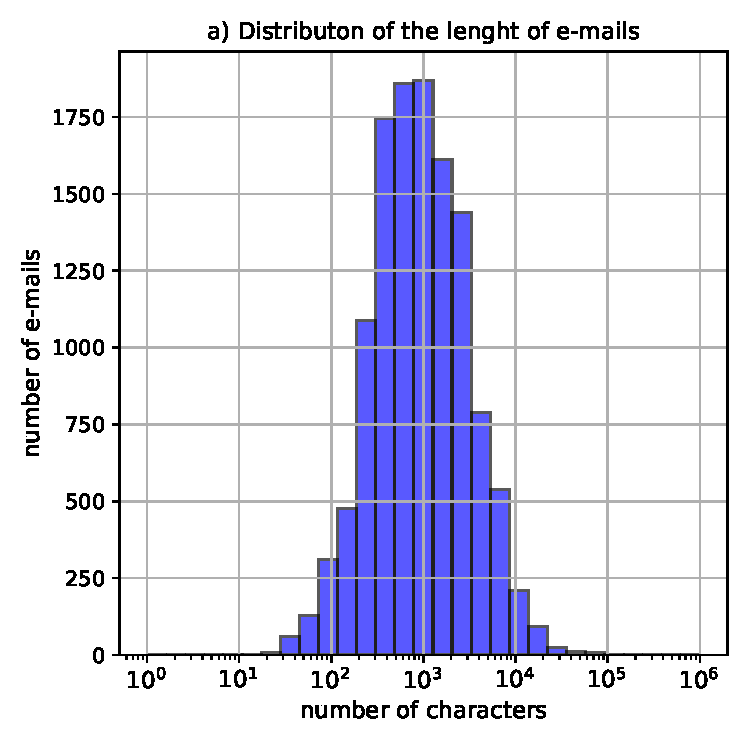
\includegraphics[width=0.35\linewidth]{char_count.pdf}}
\put(170,0){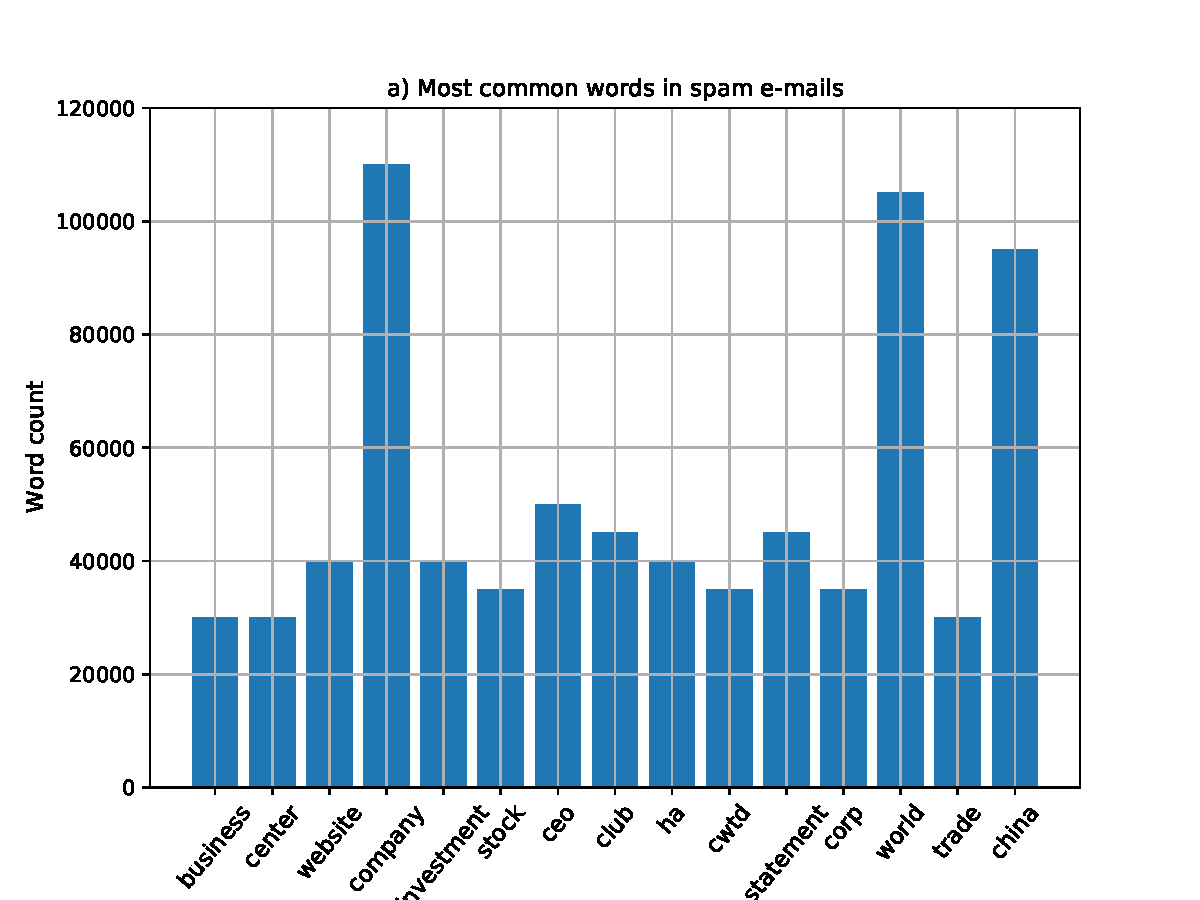
\includegraphics[width=0.35\linewidth]{spam_count.pdf}}
\put(360,0){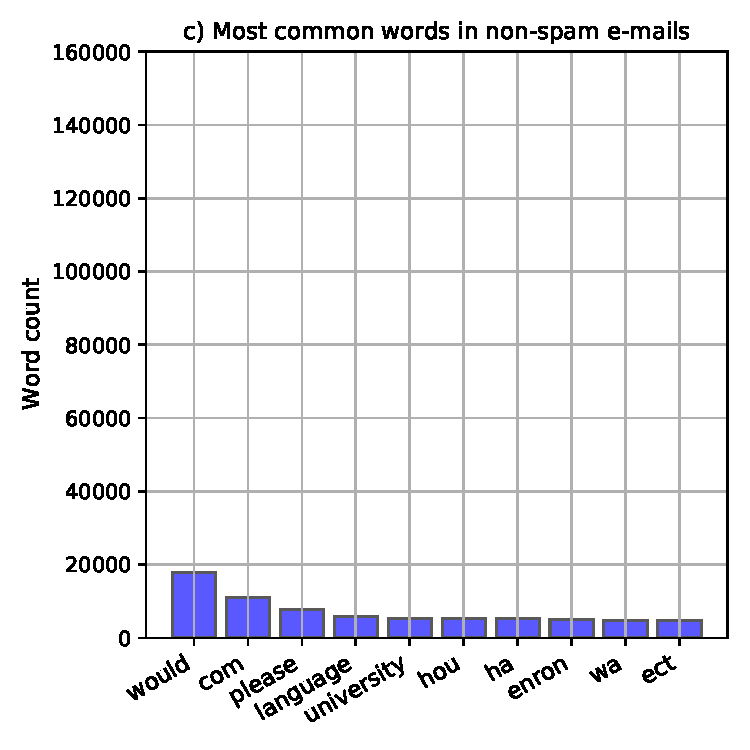
\includegraphics[width=0.35\linewidth]{ham_count.pdf}}
%\put(95,190){\textit{a})}
%\put(375,190){\textit{b})}
\end{picture}
  \caption{\textit{a}) Distribution of e-mail lenghts \textit{b})10  most common words in spam e-mails \textit{c})10 most common words in non-spam e-mails}
\label{fig::word-counts}
\end{figure}
%
We aim to apply the \textit{Bag of Words} method to the dataset. This method extracts the $N$ most common words from all e-mails and then maps an e-mail to a vector $v$, such that the component $m$ of $v$ is an non-negative integer, that counts the occurrences of the $m$th most common word in the corresponding e-mail. From that we conclude that the dimension of our dataset is $N+1$ after the bag of words transformation, since we also include the target attribute. Note that we apply the following cleanup steps to all e-mails to remove data, that we expect to not improve the classification: 1. remove links, 2. remove characters except alphabetical ones, 3. convert uppercase-chars into lowercase-chars, 4. lemmatize words 5. remove stopwords. By that we reduce the number of total distinct words in all e-mails from 126019 words to 103759 words (see jupyther notebook). This also illustrates that our classification algorithm has to work with data that is high dimensional (dimension much larger than 1000 to represent e-mails sufficiently). Since the raw data is unstructured we can't assign it to a level of measurement or dimension.       
%
In figure~\ref{fig::word-counts} b) and c) we show the most common words in spam and non-spam emails after applying our cleanup steps. One can see that the word count in spam e-mails is much higher than in the non-spam e-mails, which means that overall spam mails have more words in common than non-spam e-mails.  
%
\section{Regression Dataset: Automobile (\href{https://archive.ics.uci.edu/ml/datasets/automobile}{link to dataset})}
The automobile dataset is used for regression . It consists of 205 samples and 26 attributes where 16 attributes are given as numerical values and 10 further as nominal attributes in text form. In figure~\ref{fig::2} a) we show the numerical attributes in tabular form. In the figure we see that the symbolizing attribute is ordinal, where the others are all ratios. In the count column we note that some attributes are given for less than 205 cars, meaning that this data are missing, see also the last plot of figure~\ref{fig::3} for a distribution of missing values. For four rows the target value is missing, these rows are excluded from the data. Normalized losses has 41 missing values and will be excluded from the model. For the rest of the missing values we intend to apply a imputation technique. This is a crucial step, since the dataset is small and deleting cars with incomplete attributes would lead to significant information loss.%We can easily handle missing attributes by replacing them with the mean values over attributes.% 
  
%
\begin{figure}[H]
\begin{picture}(400,220)
\put(360,0){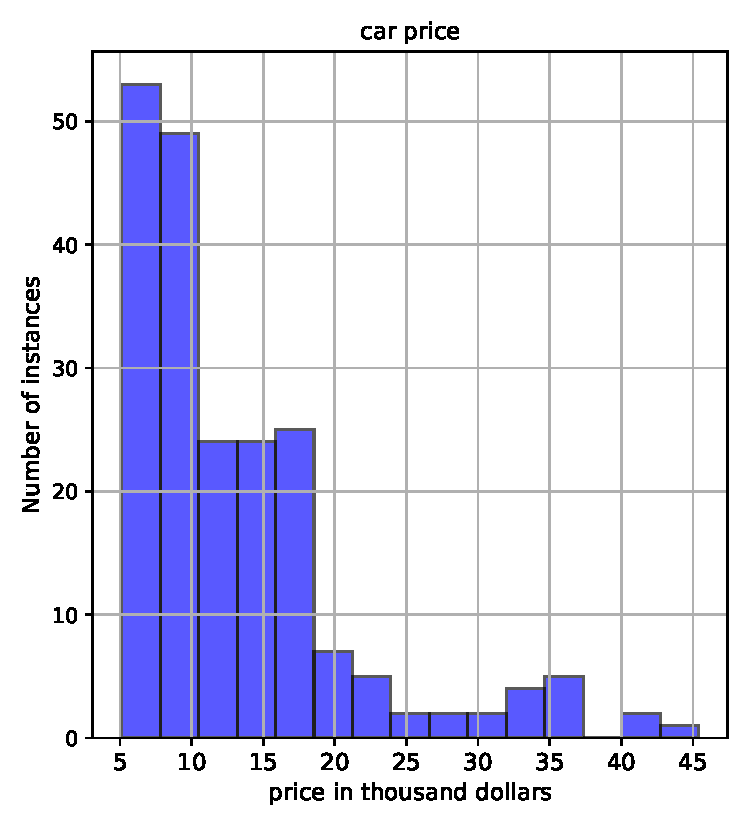
\includegraphics[width=0.35\linewidth]{car_price.pdf}}
\put(-10,100){
\footnotesize
\begin{tabular}{lrrrlrrl}
\toprule
{} &  count &     min &      max & conti &     mean &     std & attr\_type \\
\midrule
symboling          & 205 &   -2.00 &     3.00 &      False &     0.83 &    1.25 &   ordinal \\
normalized\_losses & 164 &   65.00 &   256.00 &       True &   122.00 &   35.44 &     ratio \\
wheel-base        & 205     &   86.60 &   120.90 &       True &    98.76 &    6.02 &     ratio \\
length            & 205     &  141.10 &   208.10 &       True &   174.05 &   12.34 &     ratio \\
width             & 205     &   60.30 &    72.30 &       True &    65.91 &    2.15 &     ratio \\
height            & 205     &   47.80 &    59.80 &       True &    53.72 &    2.44 &     ratio \\
curb-weight       & 205     & 1488.00 &  4066.00 &       True &  2555.57 &  520.68 &     ratio \\
engine-size       & 205     &   61.00 &   326.00 &       True &   126.91 &   41.64 &     ratio \\
bore              & 201     &    2.54 &     3.94 &       True &     3.33 &    0.27 &     ratio \\
stroke            & 201     &    2.07 &     4.17 &       True &     3.26 &    0.32 &     ratio \\
compression-ratio & 205     &    7.00 &    23.00 &       True &    10.14 &    3.97 &     ratio \\
horsepower        & 203     &   48.00 &   288.00 &       True &   104.26 &   39.71 &     ratio \\
peak-rpm          & 203     & 4150.00 &  6600.00 &       True &  5125.37 &  479.33 &     ratio \\
city-mpg          & 205     &   13.00 &    49.00 &       True &    25.22 &    6.54 &     ratio \\
highway-mpg       & 205     &   16.00 &    54.00 &       True &    30.75 &    6.89 &     ratio \\
price             & 201     & 5118.00 & 45400.00 &       True & 13207.13 & 7947.07 &     ratio \\
\bottomrule
\end{tabular}
  }
\put(180,210){\textit{a})}
\put(480,210){\textit{b})}
\end{picture}
  \caption{Numerical attributes: \textit{a}) numerical attributes of the automobile dataset \textit{b})distribution of target variable}
\label{fig::2}
\end{figure}
%
The target value for the regression is the price of a car, which is a continuous variable between $5118$ and $45400$ dollars as can be seen also in~\ref{fig::2} a). In figure~\ref{fig::2} b) the distribution of the price for a car is shown. Here we note that the price is not evenly distributed over its range and that more than 80\% of the cars cost between $5.000$ and $20.000$ dollar. Cars more expensive than $45.000$ will most likely not be predicted properly, because they are not represented in the dataset. 
%
By comparing the ranges of different numerical attributes, we note that some of them differ in orders of magnitude like the stroke and curb-weight, that differ by about two magnitudes. Therefore, we might rescale them (for example normalizing) to improve the performance of our machine learning algorithm. Note that re-scaling of the target attribute is not necessary for the most algorithms. Additionally many attributes are tail heavy, meaning their mean value differs significantly from their max and minimum sample-value. We can also try to reshape attributes that are tail-heavy into more evenly shaped distributions by a transformation to improve the performance of our algorithms.
%
The nominal attributes are plotted as histograms in figure~\ref{fig::3}. Since the nominal attributes are categorical without a defined order, we will encode them to $N$ binary attributes. %To work with nominal attributes, we aim to apply a transformation that encodes their labels in numerical values, that algorithms can easily process, this is necessary since we see that all nominal attributes have labels in textform.
%
\section{Comparison of the datasets}
%
In table~\ref{tab::1} we compare the two datasets from above.
%
\begin{figure}[H]
\begin{picture}(400,390)
\put(-20,290){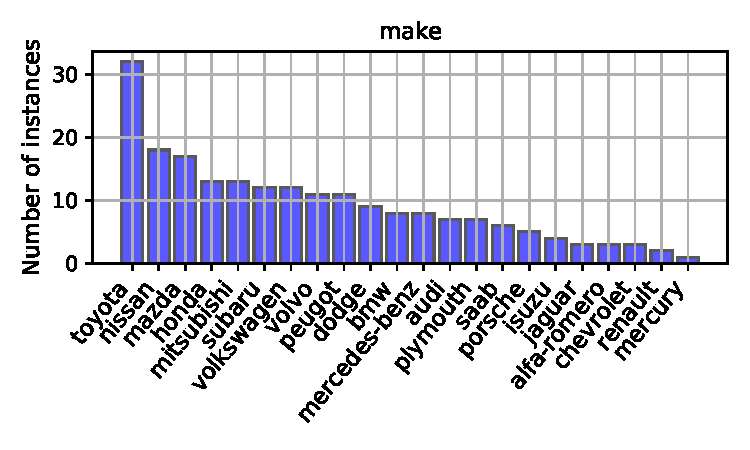
\includegraphics[width=0.35\linewidth]{car_nom1.pdf}}
\put(170,290){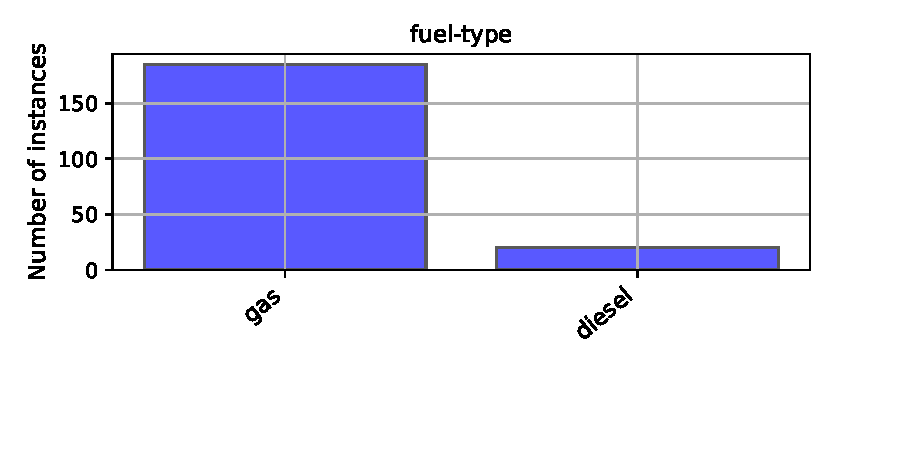
\includegraphics[width=0.35\linewidth]{car_nom2.pdf}}
\put(360,290){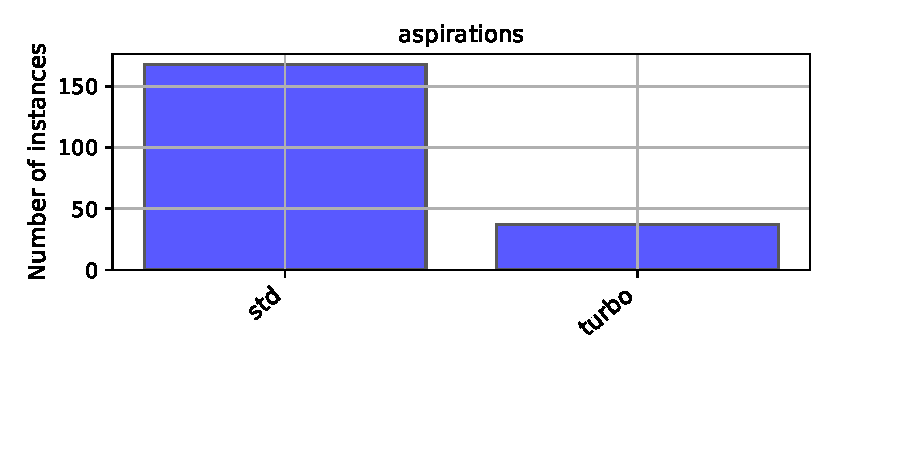
\includegraphics[width=0.35\linewidth]{car_nom3.pdf}}
\put(-20,190){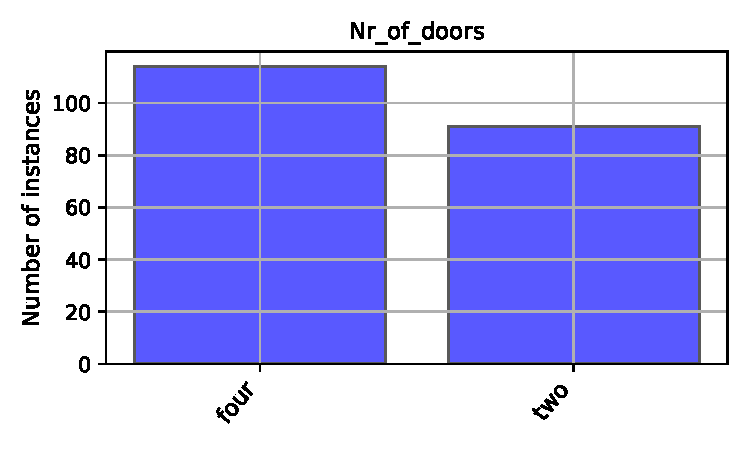
\includegraphics[width=0.35\linewidth]{car_nom4.pdf}}
\put(170,190){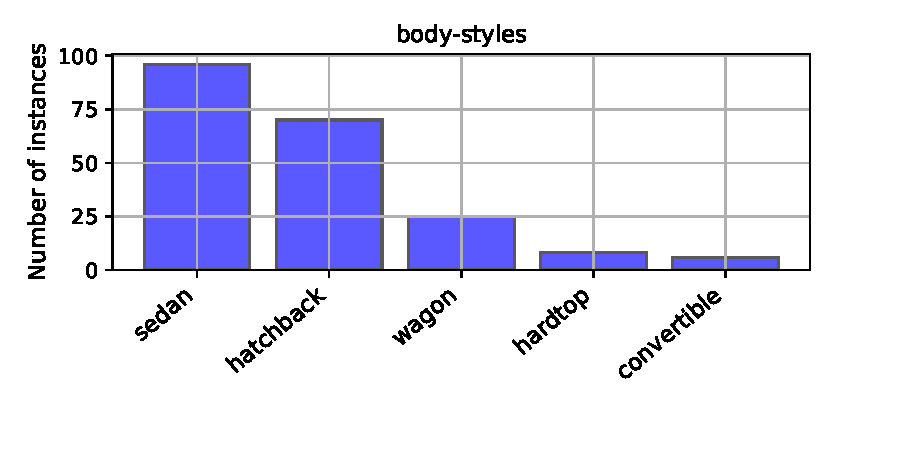
\includegraphics[width=0.35\linewidth]{car_nom5.pdf}}
\put(360,190){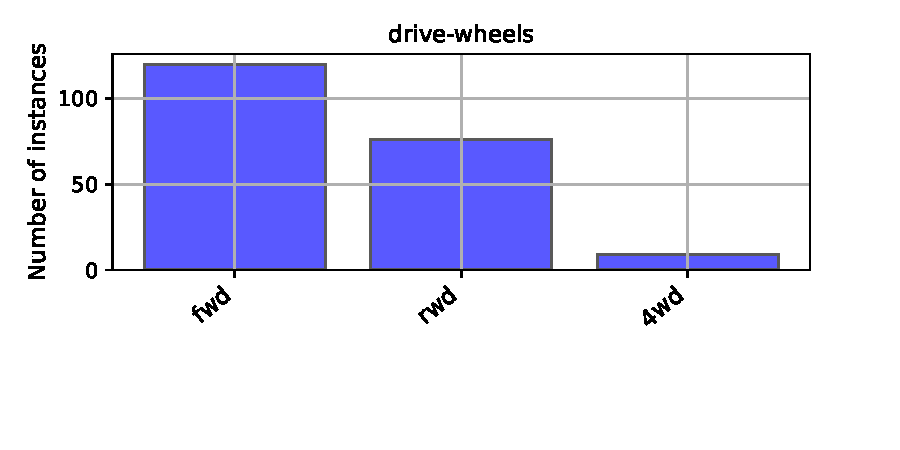
\includegraphics[width=0.35\linewidth]{car_nom6.pdf}}
\put(-20,90){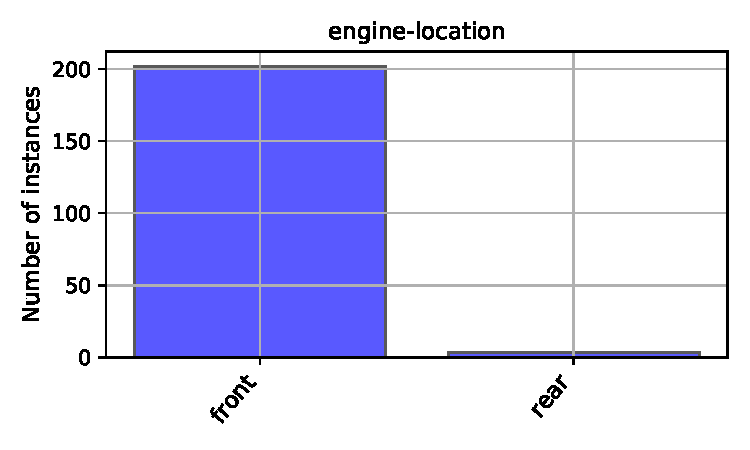
\includegraphics[width=0.35\linewidth]{car_nom7.pdf}}
\put(170,90){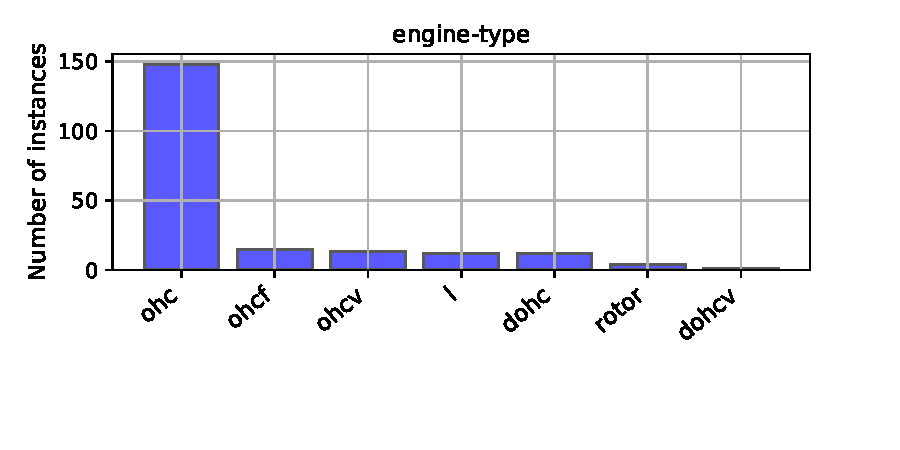
\includegraphics[width=0.35\linewidth]{car_nom8.pdf}}
\put(360,90){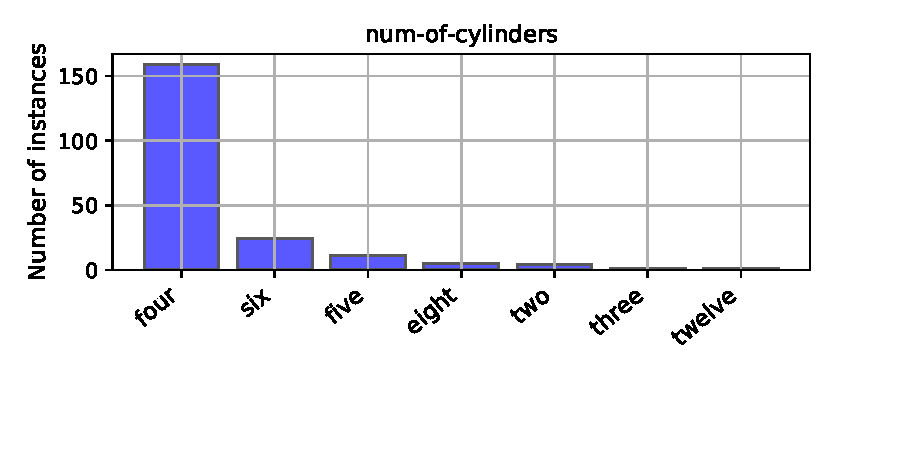
\includegraphics[width=0.35\linewidth]{car_nom9.pdf}}
\put(-20,-10){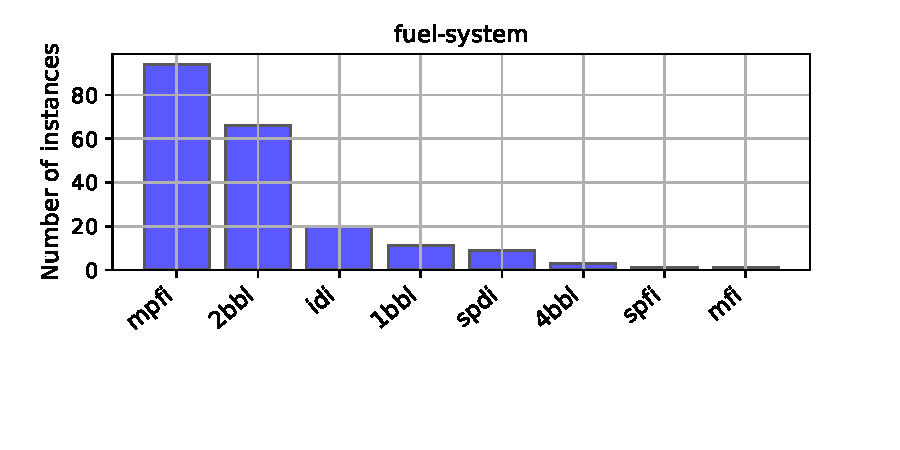
\includegraphics[width=0.35\linewidth]{car_nom10.pdf}}
\put(170,-10){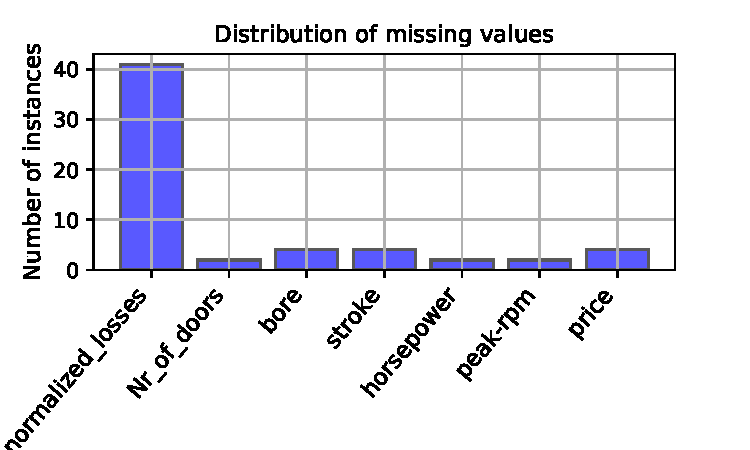
\includegraphics[width=0.35\linewidth]{car_miss.pdf}}
\end{picture}
  \caption{Nominal attributes of the automobile dataset where the last graph summarizes the missing values over all attributes}
\label{fig::3}
\end{figure}
%
%
\begin{figure}[h]
  \begin{tabular}{ | c | c | p{3cm} | c | c | c | c |}
    \hline
    Dataset     & samples & attribute-types                  & dimension  & data-types    & missing Values & duplicates \\
    \hline
    E-mail Spam & 12.277  & nominal                          & -          & text, boolean       & no  & yes\\
    \hline
    Automobile  & 205     & nominal, ordinal, intervall, ratio & 26         & integer, real, text & yes & no\\
    \hline
  \end{tabular}
    \caption{Characteristics of the chosen datasets}
    \label{tab::1}
  \end{figure}
%
Compared to the automobile dataset, the e-mail-spam dataset has about 60 times more samples,  such that we consider it as large dataset, where the automobile dataset is a small dataset. When considering the attribute-types one notes, that the automobile dataset contains all levels of measurement, where the e-mail spam dataset contains only nominal attributes. Further since the latter one is not a structured dataset it does not have a dimension, compared to the dimension of 26 in the automobile dataset. In the automobile dataset some attributes are missing, compared to the other one where no values are missing but data is duplicated.
By this we conclude that the two datasets differ greatly, as required for this exercise.
%Bibliography
\newpage
\bibliographystyle{plain}
\bibliography{Biblothek}

\end{document}
